\columnratio{0.55}
\begin{paracol}{2}

\switchcolumn[0]*%%%%%%%
\section{Lifecycle Hooks}
\switchcolumn
\section{生命周期钩子}
\switchcolumn[0]*%%%%%%%
Each Vue component instance goes through a series of initialization
steps when it's created - for example, it needs to set up data
observation, compile the template, mount the instance to the DOM, and
update the DOM when data changes. Along the way, it also runs functions
called lifecycle hooks, giving users the opportunity to add their own
code at specific stages.
\switchcolumn
每个 Vue
组件实例在创建时都需要经历一系列的初始化步骤,比如设置好数据侦听,编译模板,挂载实例到
DOM,以及在数据改变时更新
DOM。在此过程中,它也会运行被称为生命周期钩子的函数,让开发者有机会在特定阶段运行自己的代码。
\switchcolumn[0]*%%%%%%%
\subsection{Registering Lifecycle Hooks}
\switchcolumn
\subsection{注册周期钩子}


\switchcolumn[0]*%%%%%%%
For example, the \texttt{onMounted} hook can be used to run code after
the component has finished the initial rendering and created the DOM
nodes:
\switchcolumn
举例来说,\texttt{onMounted} 钩子可以用来在组件完成初始渲染并创建 DOM
节点后运行代码:
\switchcolumn[0]*%%%%%%%
\begin{codeHtml}
<script setup>
import { onMounted } from 'vue'
<!-- -->
onMounted(() => {
  console.log(`the component is now mounted.`)
})
</script>
\end{codeHtml}
\switchcolumn
\begin{codeHtml}
<script setup>
import { onMounted } from 'vue'
<!-- -->
onMounted(() => {
  console.log(`the component is now mounted.`)
})
</script>
\end{codeHtml}
\switchcolumn[0]*%%%%%%%
There are also other hooks which will be called at different stages of
the instance's lifecycle, with the most commonly used being
\href{https://vuejs.org/api/composition-api-lifecycle.html\#onmounted}{\texttt{onMounted}},
\href{https://vuejs.org/api/composition-api-lifecycle.html\#onupdated}{\texttt{onUpdated}},
and
\href{https://vuejs.org/api/composition-api-lifecycle.html\#onunmounted}{\texttt{onUnmounted}}.
\switchcolumn
还有其他一些钩子,会在实例生命周期的不同阶段被调用,最常用的是
\href{https://cn.vuejs.org/api/composition-api-lifecycle.html\#onmounted}{\texttt{onMounted}}、\href{https://cn.vuejs.org/api/composition-api-lifecycle.html\#onupdated}{\texttt{onUpdated}}
和
\href{https://cn.vuejs.org/api/composition-api-lifecycle.html\#onunmounted}{\texttt{onUnmounted}}。所有生命周期钩子的完整参考及其用法请参考
\href{https://cn.vuejs.org/api/composition-api-lifecycle.html}{API
索引}。


\switchcolumn[0]*%%%%%%%
When calling \texttt{onMounted}, Vue automatically associates the
registered callback function with the current active component instance.
This requires these hooks to be registered \textbf{synchronously} during
component setup. For example, do not do this:
\switchcolumn
当调用 \texttt{onMounted} 时,Vue
会自动将回调函数注册到当前正被初始化的组件实例上。这意味着这些钩子应当在组件初始化时被\textbf{同步}注册。例如,请不要这样做:
\switchcolumn[0]*%%%%%%%
\begin{codeJs}
setTimeout(() => {
  onMounted(() => {
    // 异步注册时当前组件实例已丢失
    // 这将不会正常工作
  })
}, 100)
\end{codeJs}
\switchcolumn
\begin{codeJs}
setTimeout(() => {
  onMounted(() => {
    // 异步注册时当前组件实例已丢失
    // 这将不会正常工作
  })
}, 100)
\end{codeJs}
\switchcolumn[0]*%%%%%%%
Do note this doesn't mean that the call must be placed lexically inside
\texttt{setup()} or \texttt{\textless{}script\ setup\textgreater{}}.
\texttt{onMounted()} can be called in an external function as long as
the call stack is synchronous and originates from within
\texttt{setup()}.
\switchcolumn
注意这并不意味着对 \texttt{onMounted} 的调用必须放在 \texttt{setup()} 或
\texttt{\textless{}script\ setup\textgreater{}}
内的词法上下文中。\texttt{onMounted()}
也可以在一个外部函数中调用,只要调用栈是同步的,且最终起源自
\texttt{setup()} 就可以。


\switchcolumn[0]*%%%%%%%
\subsection{Lifecycle Diagram}
\switchcolumn
\subsection{生命周期图示}
\switchcolumn[0]*%%%%%%%
Below is a diagram for the instance lifecycle. You don't need to fully
understand everything going on right now, but as you learn and build
more, it will be a useful reference.
\switchcolumn
下面是实例生命周期的图表。你现在并不需要完全理解图中的所有内容,但以后它将是一个有用的参考。
\end{paracol}

\begin{center} 
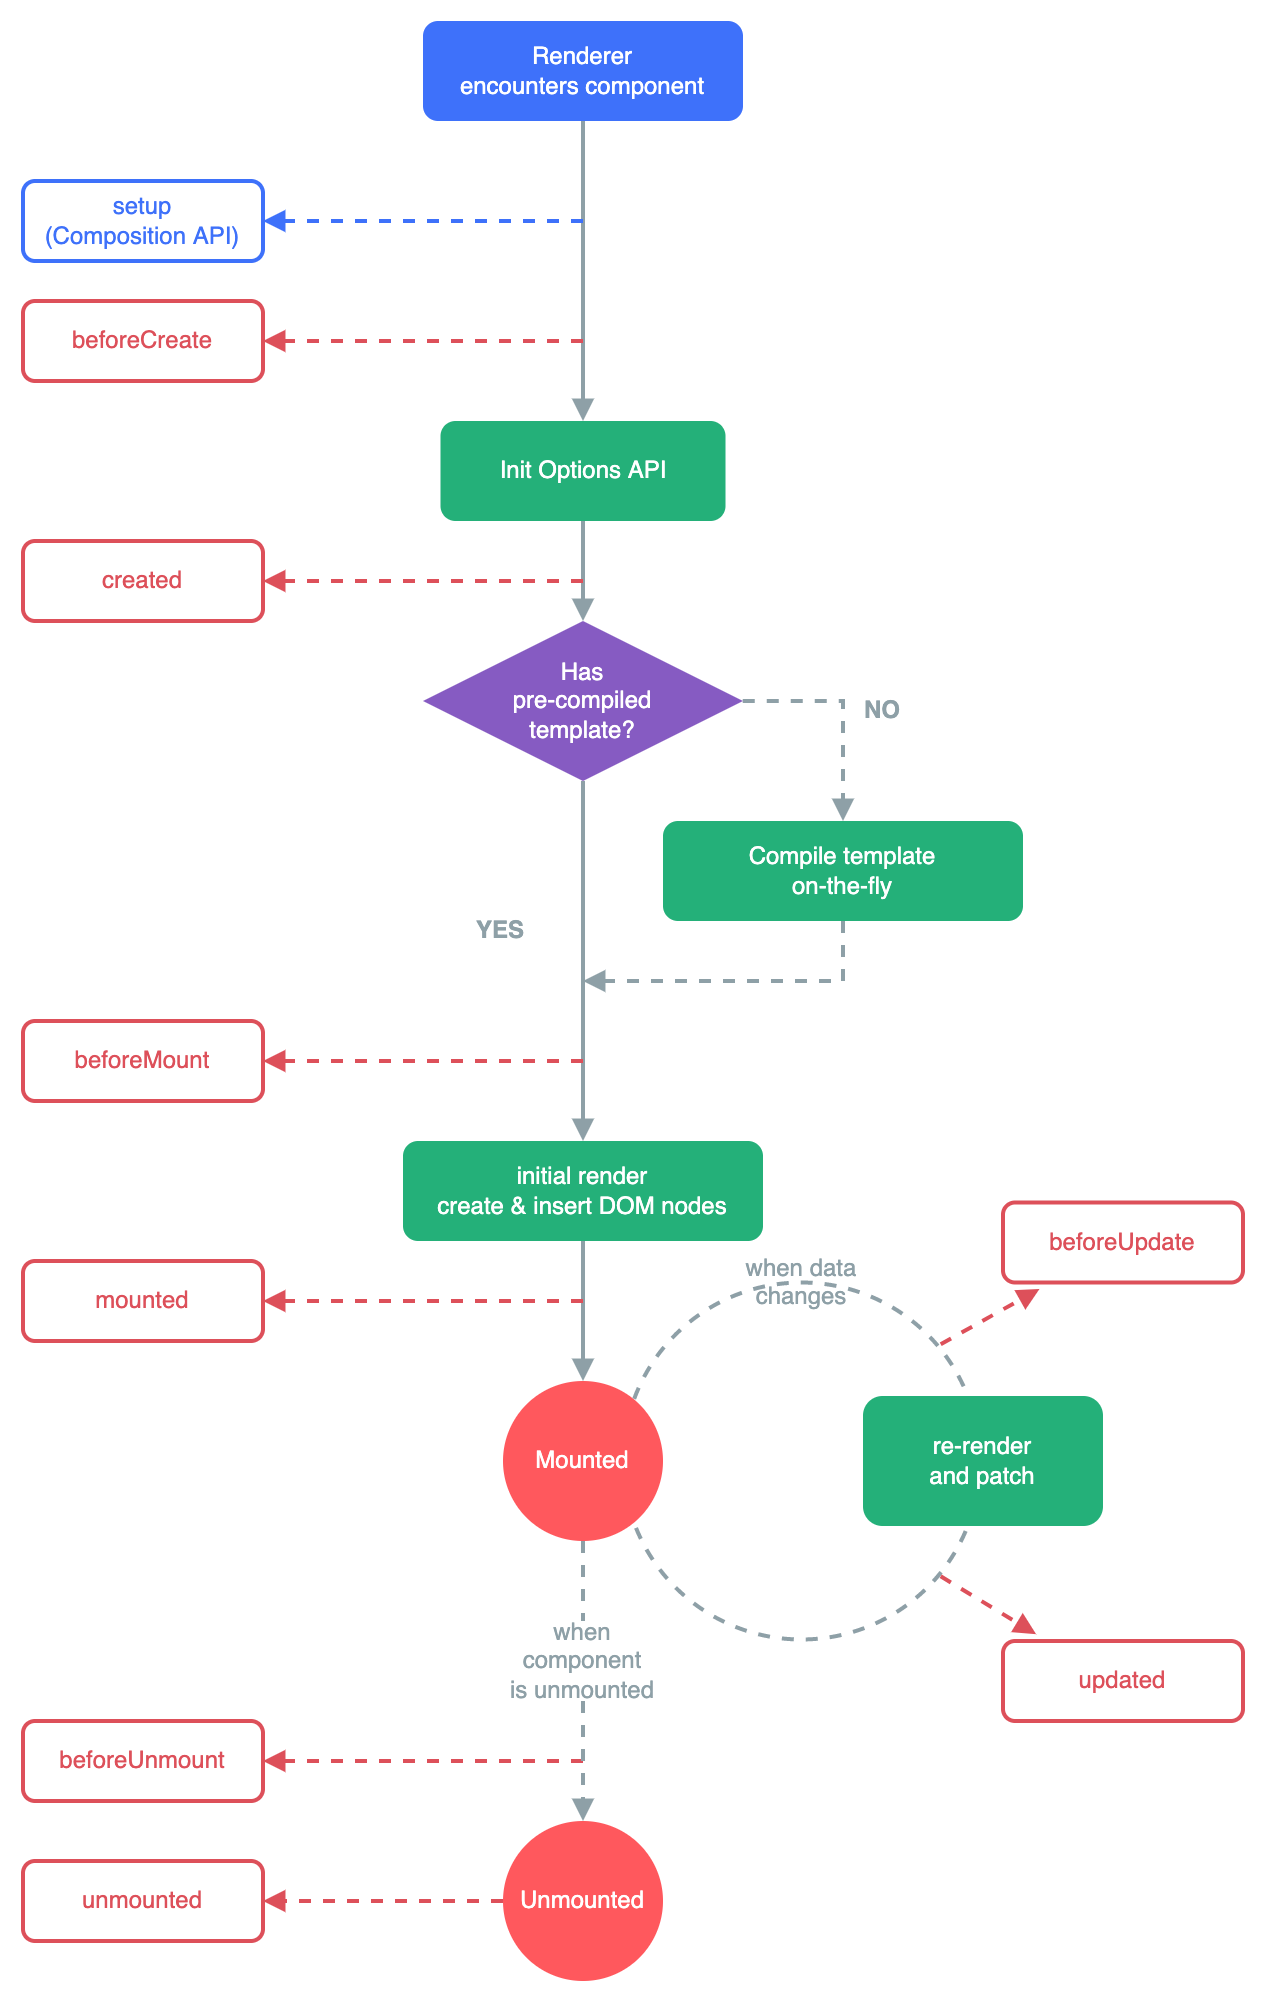
\includegraphics[scale=0.3]{./img/lifecycle.16e4c08e.png} 
\end{center}

\columnratio{0.55}
\begin{paracol}{2}
\switchcolumn[0]*%%%%%%%
Consult the
\href{https://vuejs.org/api/composition-api-lifecycle.html}{Lifecycle
Hooks API reference} for details on all lifecycle hooks and their
respective use cases.
\switchcolumn
有关所有生命周期钩子及其各自用例的详细信息,请参考\href{https://cn.vuejs.org/api/composition-api-lifecycle.html}{生命周期钩子
API 索引}。
\end{paracol}


